\documentclass{article}
\usepackage{fancyhdr}
\usepackage{titlesec}
\usepackage{listings}
\usepackage{xcolor}
\usepackage{enumitem}
\usepackage{graphicx}
\usepackage{lmodern}
\graphicspath{ {./img/} }

% Define colors for syntax highlighting
\definecolor{codegreen}{rgb}{0,0.6,0}
\definecolor{codegray}{rgb}{0.5,0.5,0.5}
\definecolor{stringyellow}{rgb}{0.8,0.8,0} % New yellow color for strings
\definecolor{backcolour}{rgb}{0.95,0.95,0.92}
\definecolor{keywordblue}{rgb}{0,0,0.8}

% Configure listing style for perfect alignment
\lstdefinestyle{paragraphstyle}{
    backgroundcolor=\color{backcolour},
    commentstyle=\color{codegreen},
    keywordstyle=\color{keywordblue},
    numberstyle=\tiny\color{codegray},
    stringstyle=\color{stringyellow}, % Changed from purple to yellow
    basicstyle=\ttfamily\small,
    breakatwhitespace=false,
    breaklines=true,
    captionpos=b,
    keepspaces=true,
    numbers=none,
    showspaces=false,
    showstringspaces=false,
    showtabs=false,
    tabsize=2,
    xleftmargin=0pt,
    xrightmargin=0pt,
    framexleftmargin=0pt,
    framexrightmargin=0pt,
    frame=single,
    framesep=3pt,
}


\lstset{style=paragraphstyle}

\pagestyle{fancy}
\fancyhf{}
\lhead{Modul 1 Praktikum Bioinformatika}
\rfoot{\footnotesize Page \thepage}
\lfoot{\footnotesize Dr. Muhammad Subianto, M.Si, Ir. Essy Harnelly, S.Si., M.Si., Ph.D., Imelda Meilani, S.Si., M.Si.\newline Jurusan Informatika Universitas Syiah Kuala \newline Modul oleh :  Rendika Rahmaturrizki}
\renewcommand{\headrulewidth}{1pt}
\renewcommand{\footrulewidth}{1pt}

\titleformat*{\section}{\small\bfseries}

\begin{document}
    \begin{center}  
        \textbf{Modul 1 Praktikum Jaringan Komputer}

        \textbf{Perkenalan Jaringan Komputer}
    \end{center}

    \section*{Deskripsi Singkat}
   Praktikum Bioinformatika adalah praktikum untuk menunjang mata kuliah Bioinformatika. Praktikum ini menggunakan data molekuler seperti DNA, protein,dll. dan bahasa pemrograman Python. Materi praktikum akan berisi tutorial, latihan dan soal.
   

    \section*{Tujuan}
    \begin{enumerate}
        \item Dapat menggunakan Database Molekuler dengan terampil
        \item Dapat menggunakan file FASTA dan sejenisnya dengan baik
    \end{enumerate}

    \begin{flushleft}
        \textbf{Materi 1 - Database Molekuler}
        \newline

        \begin{enumerate}
            \item NCBI
            
            NCBI (National Centre for Biotechnology Information) merupakan sebuah
            institusi yang memiliki konsentrasi dalam perkembangan ilmu Biologi Molekuler.
            Salah satu dari fitur yang dikembangkan NCBI adalah GenBank. GenBank menyediakan lebih dari 610,000 jenis spesies dalam bentuk urutan nukleotida dengan melakukan pembaruan data yang sekarang terdapat 318,618 sequence record dan 441,315,689,217 base pairs data baru dan juga disinkronisasikan dengan ENA (European Nucleotide Archive) dan DDJB (DNA Data Bank of Japan) sehingga datanya telah mencakupi seluruh wilayah di dunia.
            \par\vspace{0.5cm} 
            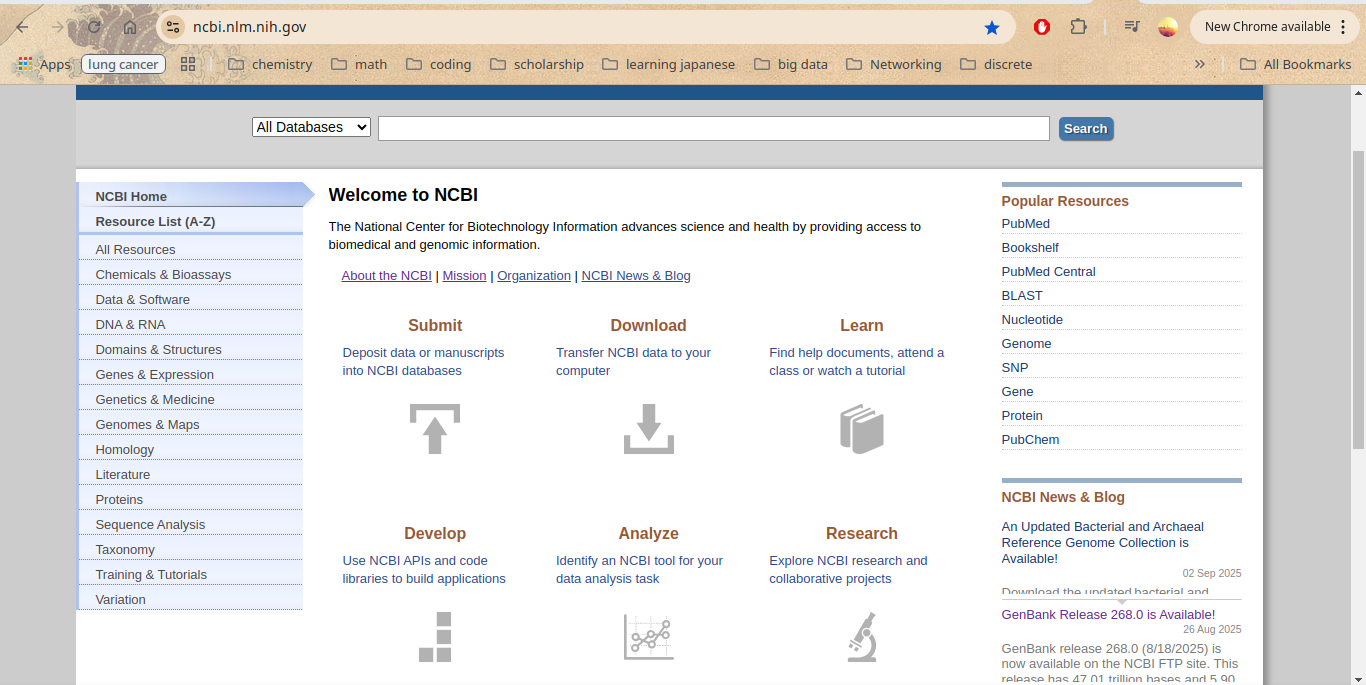
\includegraphics[scale=0.3]{Modul1/img/1.png}
           
            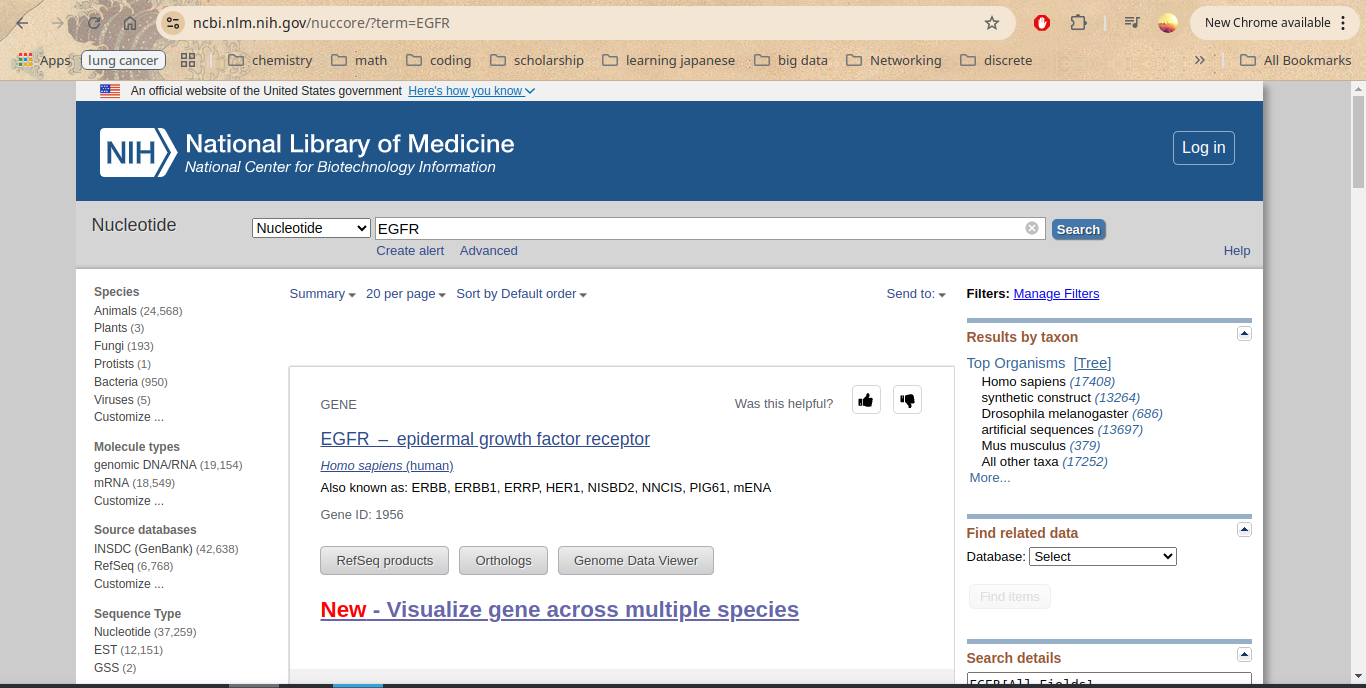
\includegraphics[scale=0.3]{Modul1/img/2.png}

            \item EMBL-EBI / ENA (European Nucleotide Archive)

            EMBL (European Molecular Biology Laboratory) adalah salah satu lembaga
            non-profit yang melakukan penelitian ilmu kehidupan dan pengembangan biologi
            molekuler. Salah satu bagiannya adalah EMBL-EBI (European Bioinformatics
            Institute) yang mengumpulkan berbagai informasi biologi molekuler. EMBL-EBI mengelola rangkaian sumber daya dan alat data yang paling komprehensif di dunia yang tersedia secara bebas. Hal ini sangat penting untuk penelitian, penemuan, dan pengembangan solusi inovatif terhadap tantangan global seperti kesehatan manusia, kerawanan pangan, dan hilangnya keanekaragaman hayati.
            \par\vspace{0.5cm} 
            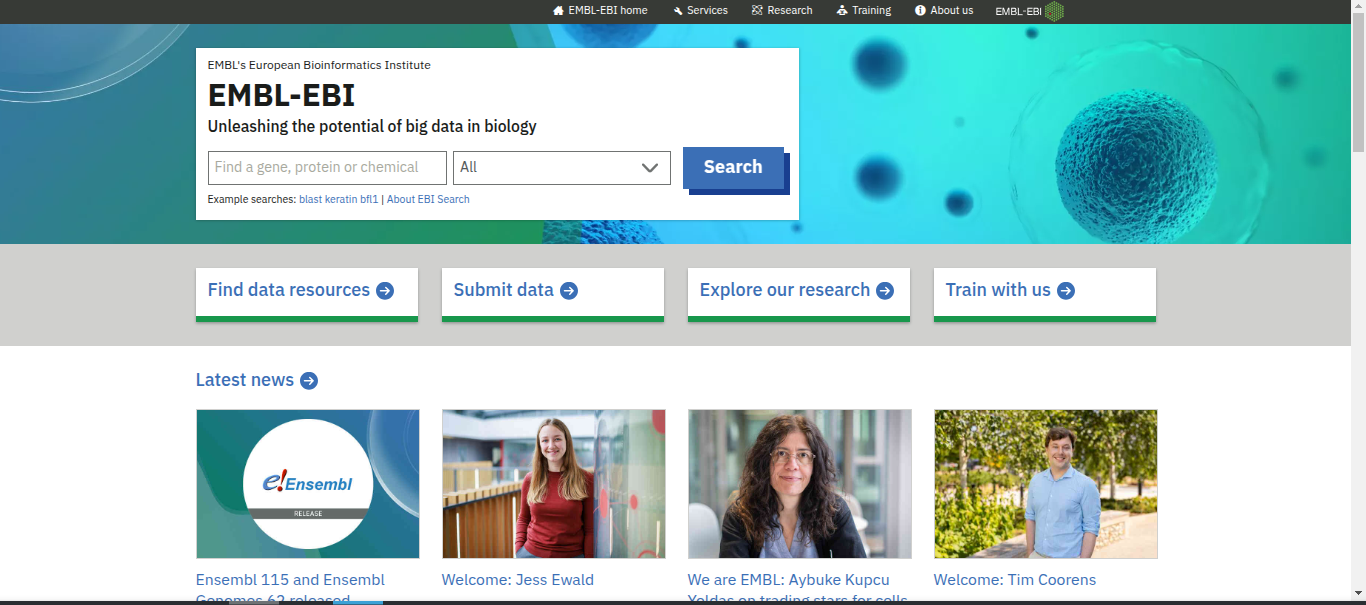
\includegraphics[scale=0.3]{Modul1/img/3.png}

            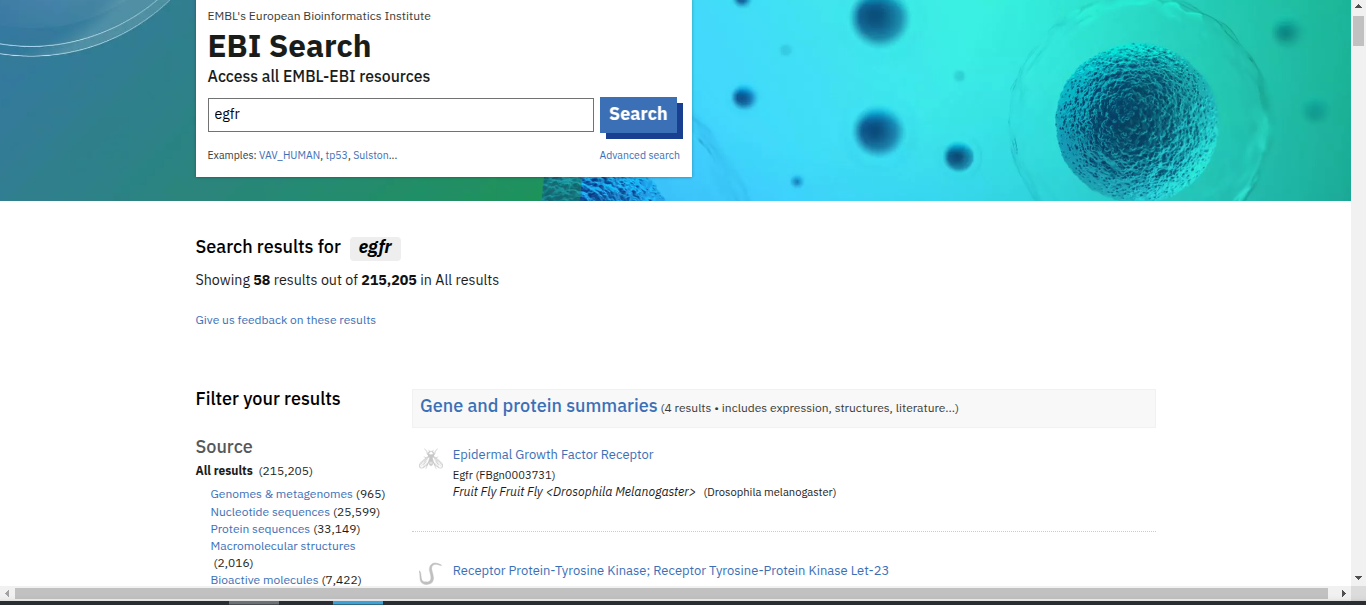
\includegraphics[scale=0.3]{Modul1/img/4.png}

            \item DDBJ

            DDBJ (DNA Data Bank of Japan) adalah bank data yang di National Institute
            of Genetics (NIG) yang berlokasi di Mishima, Jepang, sebagai bagian dari
            Internasional Nucleotide Sequence Database (INSDC) yang bekerja sama dengan
            NCBI dan EMBL-EBI. Ketiga bank data ini saling bertukar data yang hampir sama.
            DDJB menyediakan berbagai sekuen nukleotida baik yang berasal dari berbagai
            wilayah baik Jepang ataupun negara-negara lainnya.
            \par\vspace{0.5cm}
            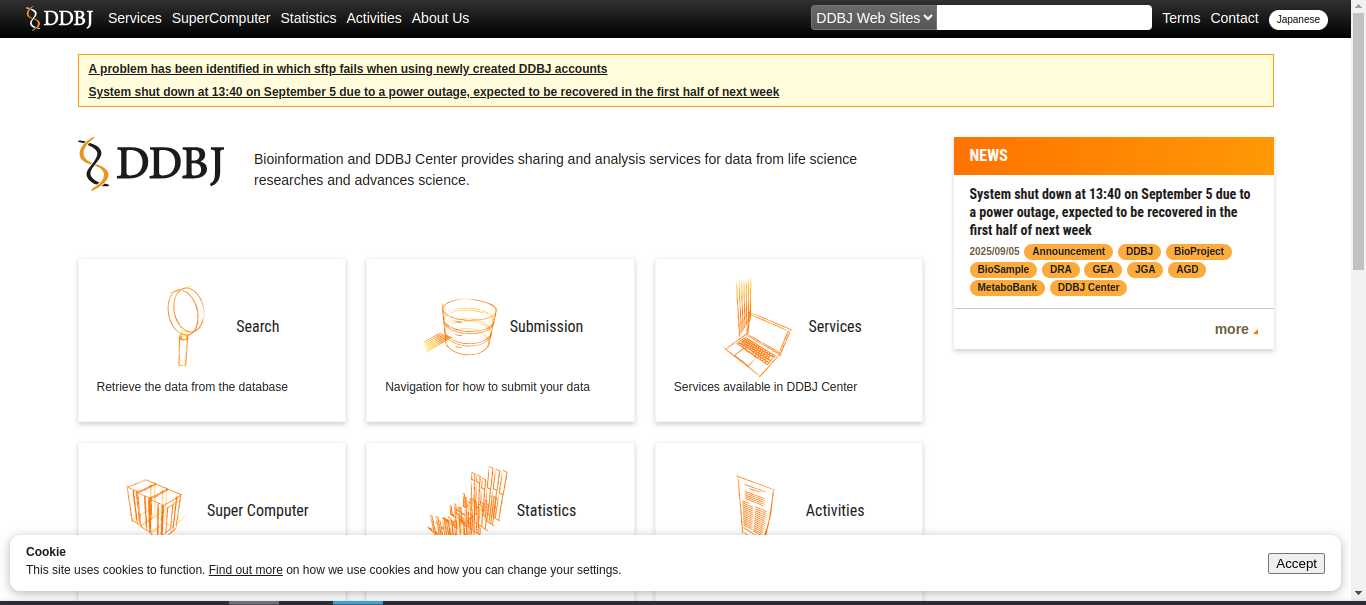
\includegraphics[scale=0.3]{Modul1/img/5.png}

            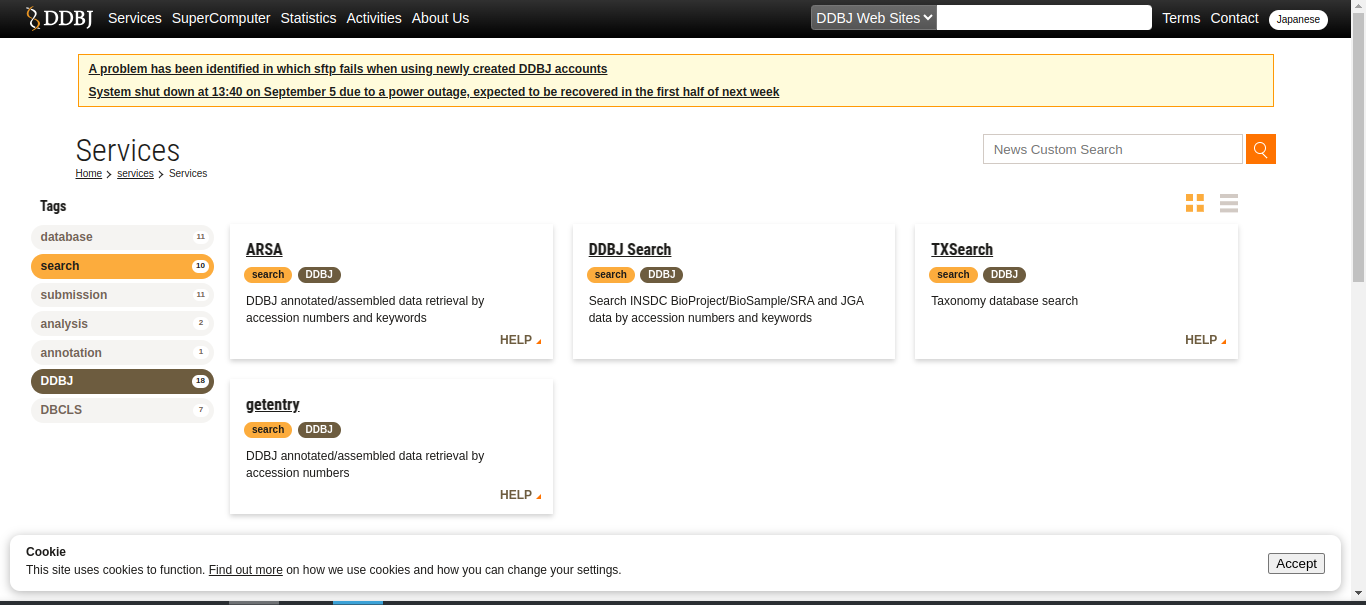
\includegraphics[scale=0.3]{Modul1/img/6.png}

            \item EpiCoV GISAID

            GISAID merupakan bank data yang melingkupi semua jenis virus influenza,
            Respiratory Syntical Virus (RSV) hingga sindrom pernafasan akut coronavirus 2019
            (Covid-19). Platform ini dapat diakses secara publik dengan 42.000 peneliti dari 198
            negara dan lebih dari 3500 institusi di seluruh dunia. Situs ini sangat berjasa dalam
            perkembangan ilmu terutama di masa pandemi virus saat ini. Sejak sekuen genom
            pertama yang diunggah oleh CDC China pada 10 Januari 2020, sudah lebih dari 5
            juta sekuens genetik SARS-CoV-2 dari 194 negara dan wilayah tersedia melalui
            bank data EpiCoV GISAID.
            \par\vspace{0.5cm}
            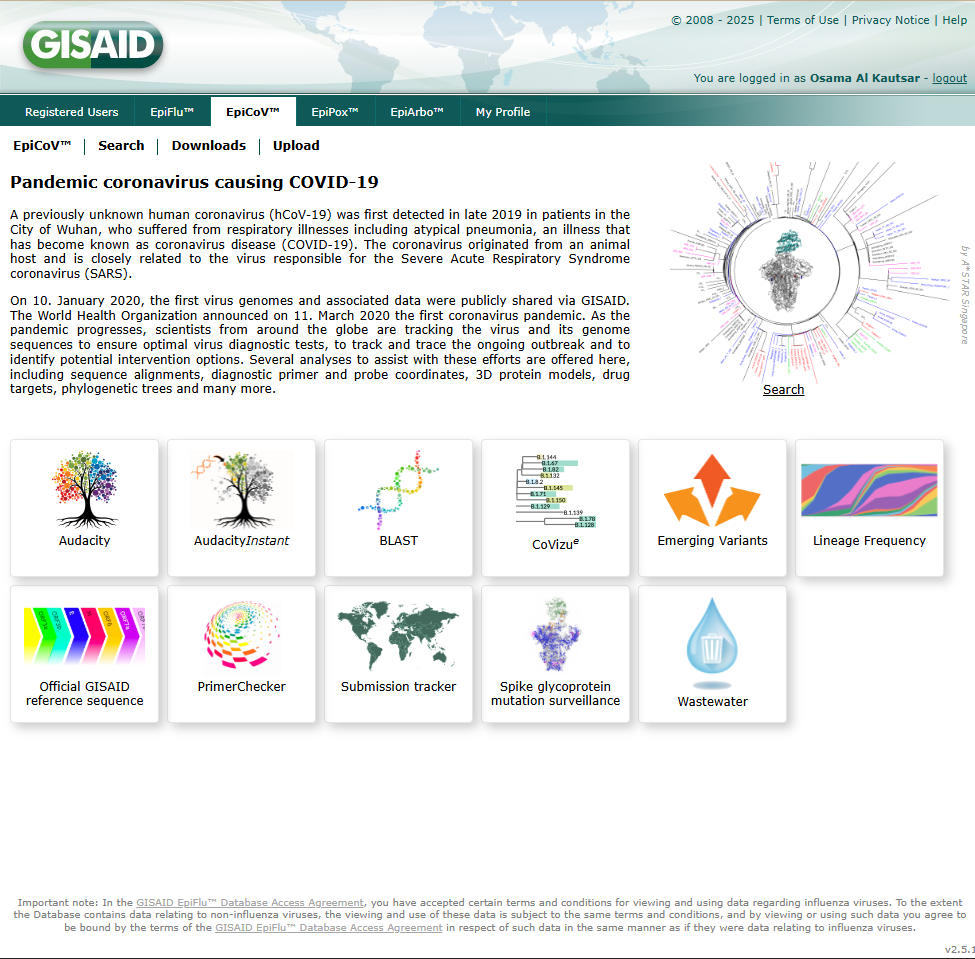
\includegraphics[scale=0.4]{Modul1/img/7.png}

            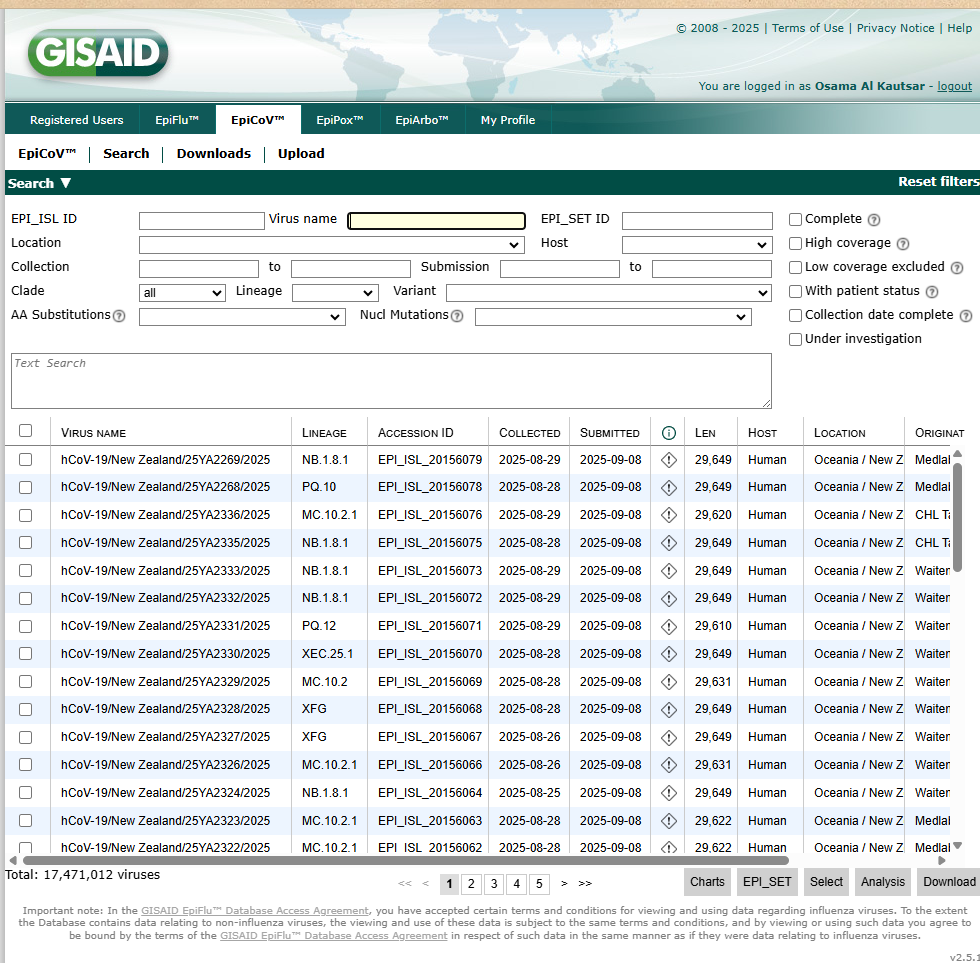
\includegraphics[scale=0.4]{Modul1/img/8.png}

            \item UniProtKB / Swiss-Prot

            UniProtKB merupakan hasil konsorsium hasil kerja sama antara Swiss Institute
            of Bioinformatics (SIB) dan European Bioinformatics Institute (EBI), yang bertujuan
            untuk menyediakan komunitas ilmiah yang berada di satu pusat untuk data urutan
            protein dan beberapa informasi fungsional. Situs ini menyediakan berbagai data urutan protein dari berbagai jenis spesies hewan, tumbuhan hingga mikroba.
            \par\vspace{0.5cm}
            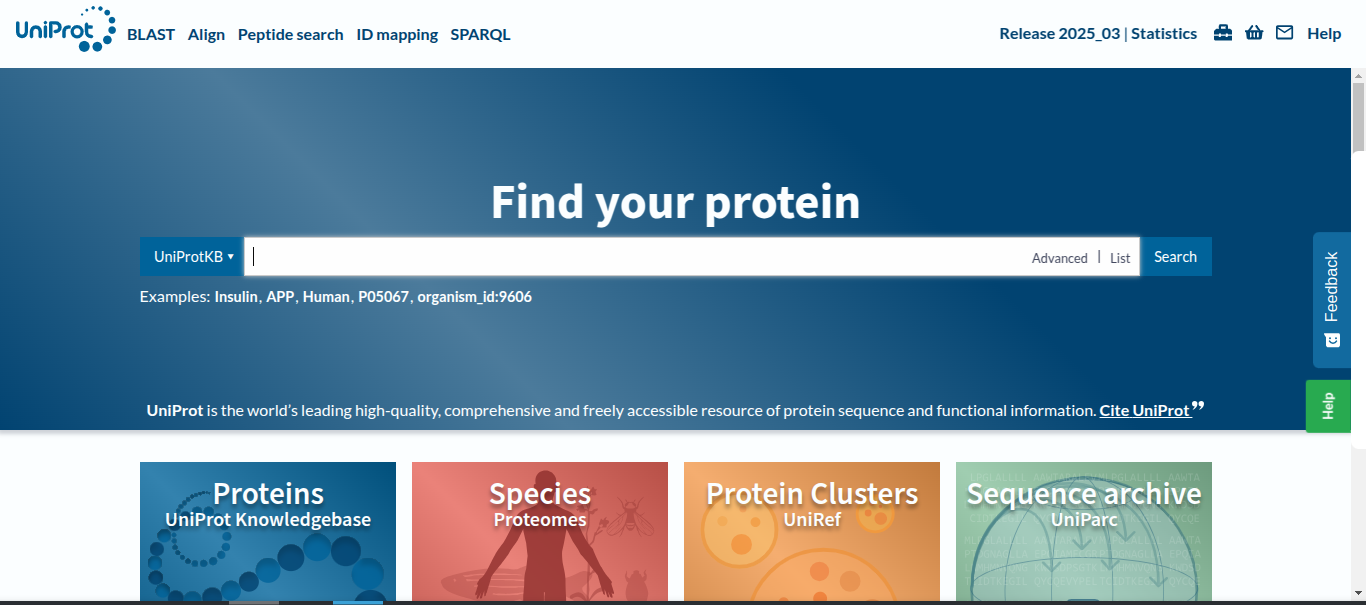
\includegraphics[scale=0.3]{Modul1/img/9.png}

            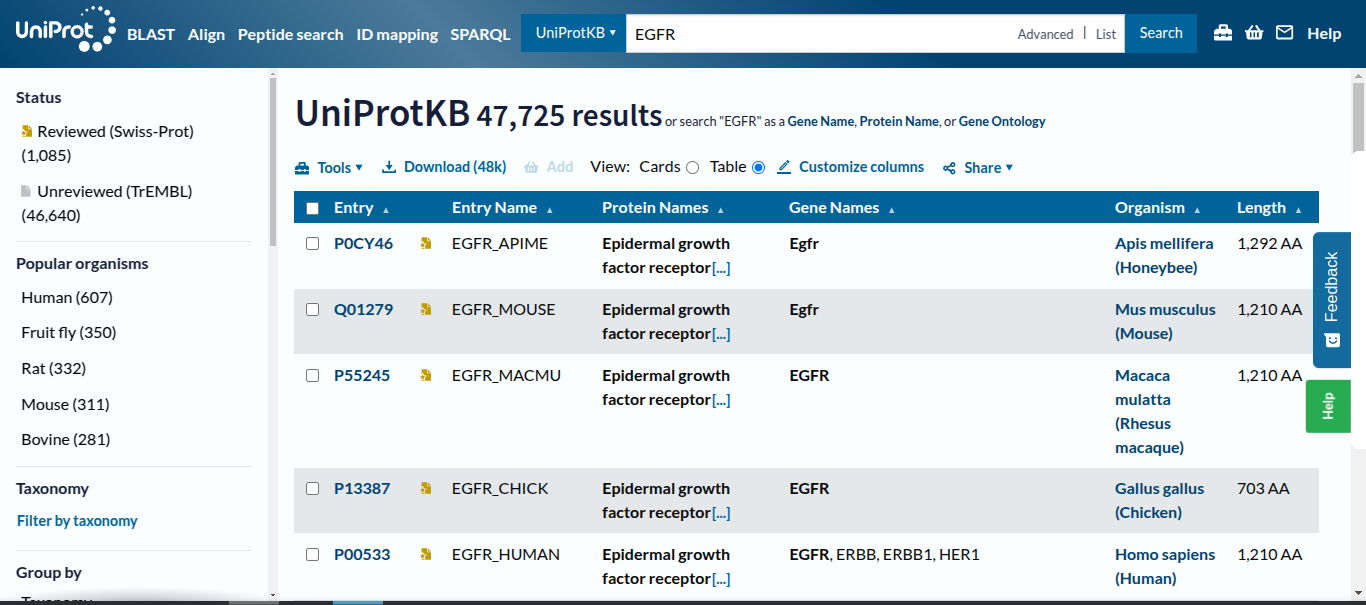
\includegraphics[scale=0.3]{Modul1/img/10.png}

            \item RCSB-PDB

            Protein Data Bank (PDB) merupakan kumpulan arsip tunggal mengenai data
            struktural makromolekul biologi dari seluruh dunia. Penentuan struktur molekul protein yang terdapat pada berkas PDB diperoleh dengan menggunakan data eksperimen. Data eksperimen ini berasal dari kristalografi sinar-x atau spektroskopi Nuclear Magnetic Resonance (NMR), kemudian dilakukan proses dengan program komputer untuk membuat model molekul yang paling sesuai dengan data eksperimen. Situs PDB dapat diakses pada alamat www.rcsb.org. Situs ini dapat diakses oleh seluruh pengguna internet di seluruh dunia secara gratis. PDB merupakan suatu proyek pendataan makromolekul biokimia (seperti protein dan asam nukelat) yang dikembangkan oleh Research Collaboratory for Structural Bioinformatics (RCSB). Format file ini memiliki ekstensi (.pdb.).
            \par\vspace{0.5cm}
            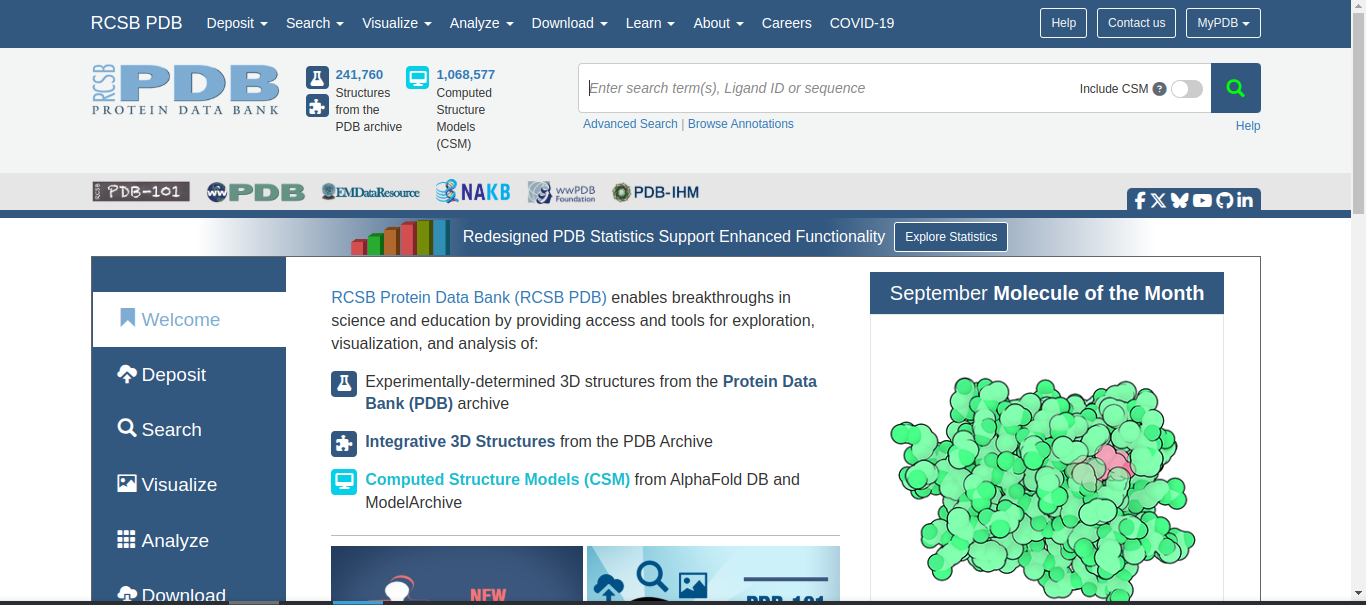
\includegraphics[scale=0.3]{Modul1/img/11.png}

            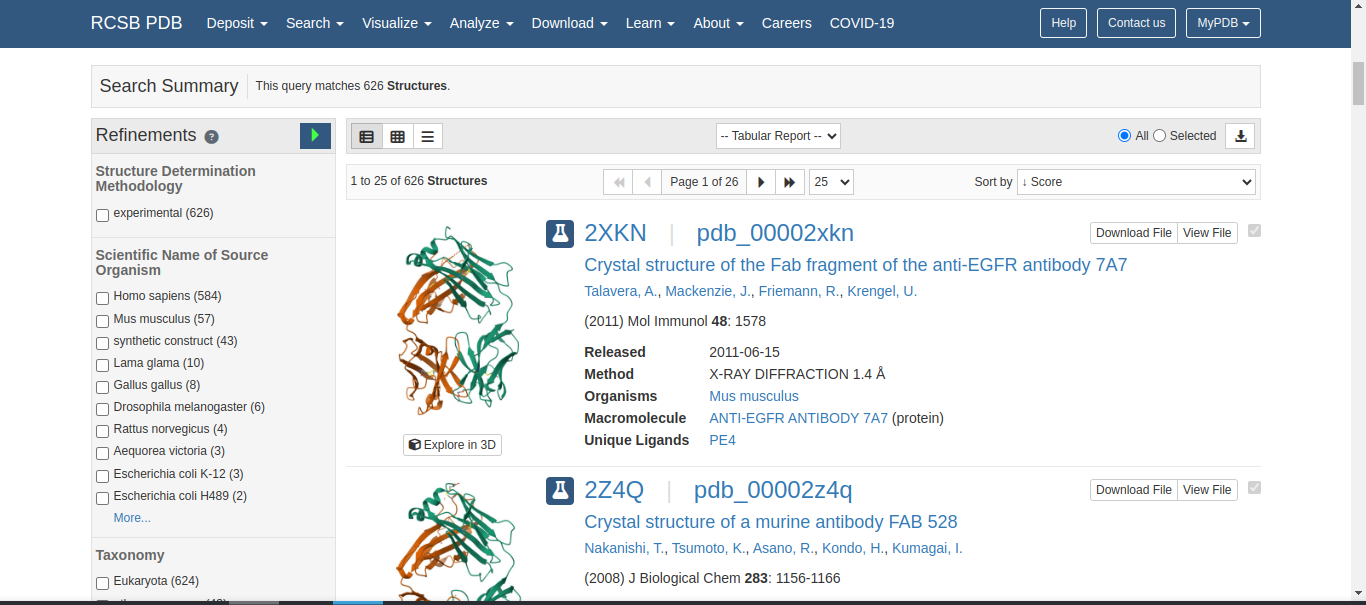
\includegraphics[scale=0.3]{Modul1/img/12.png}      
        \end{enumerate}
            Cara penggunaan NCBI adalah sebagai berikut:
            \begin{enumerate}
                \item Cari nama gen yang ingin dicari dan pastikan untuk memilih jenis tipe data yang ingin dicari (dalam contoh ini berupa nukleotida)
                \par\vspace{0.5cm}
                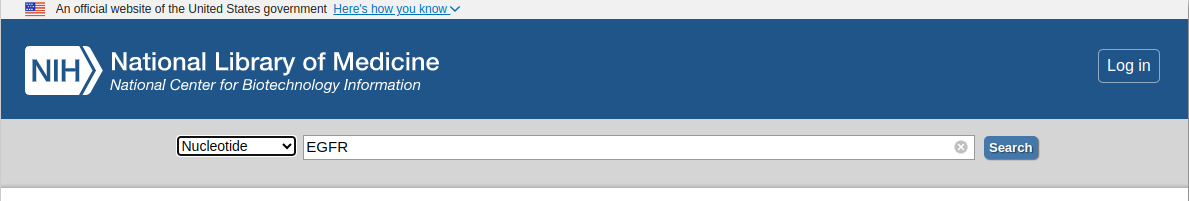
\includegraphics[scale=0.3]{Modul1/img/13.png}

                \item Lalu setelah keluar hasil pencarian, pilih gen yang sesuai dengan yang anda cari
                \par\vspace{0.5cm}
                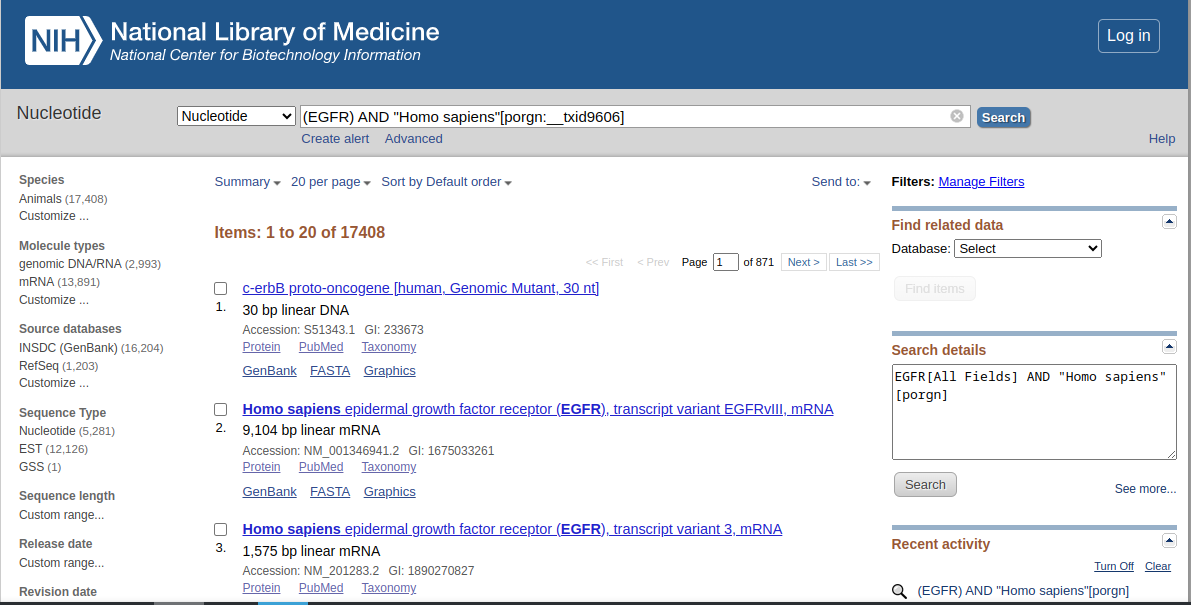
\includegraphics[scale=0.3]{Modul1/img/14.png}

                \item Akan keluar halaman deskripsi mengenai gen tersebut yang anda pilih, terdapat accession ID yang merupakan ID unik setiap sequence records
                \par\vspace{0.5cm}
                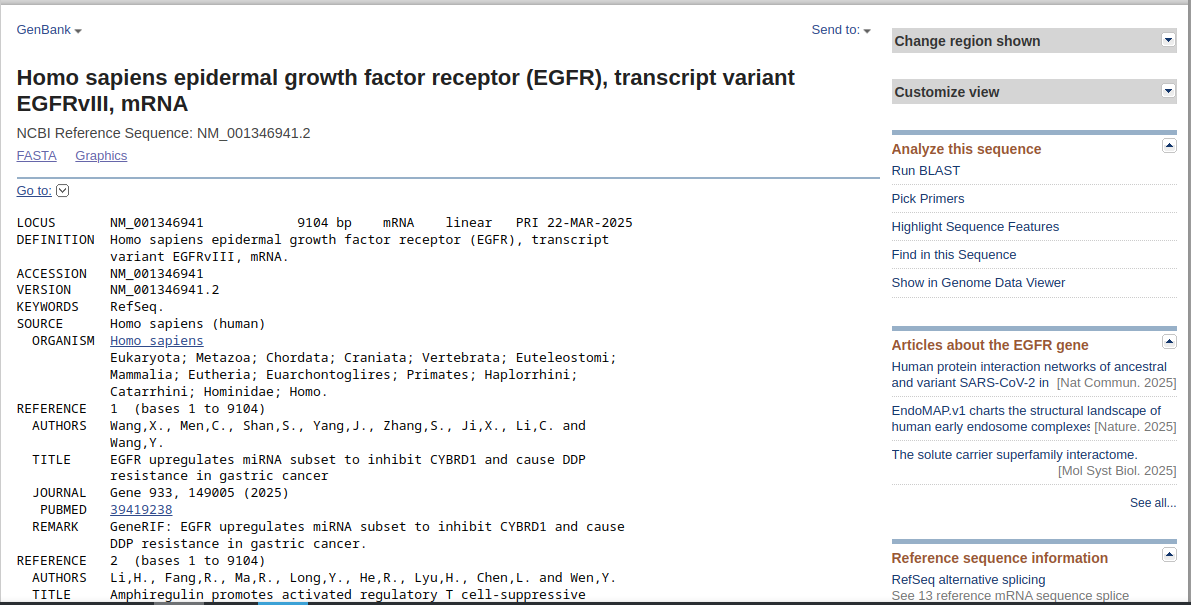
\includegraphics[scale=0.3]{Modul1/img/15.png}

                \item Untuk mengunduh data tersebut pertama perlu klik pada  Send to,  lalu pilih jenis filenya berupa Complete Record,  lalu pilih tujuannya berupa File , dan pilih format nya berupa file FASTA, lalu Create File, dan simpan outputnya di perangkat anda
                \par\vspace{0.5cm}
                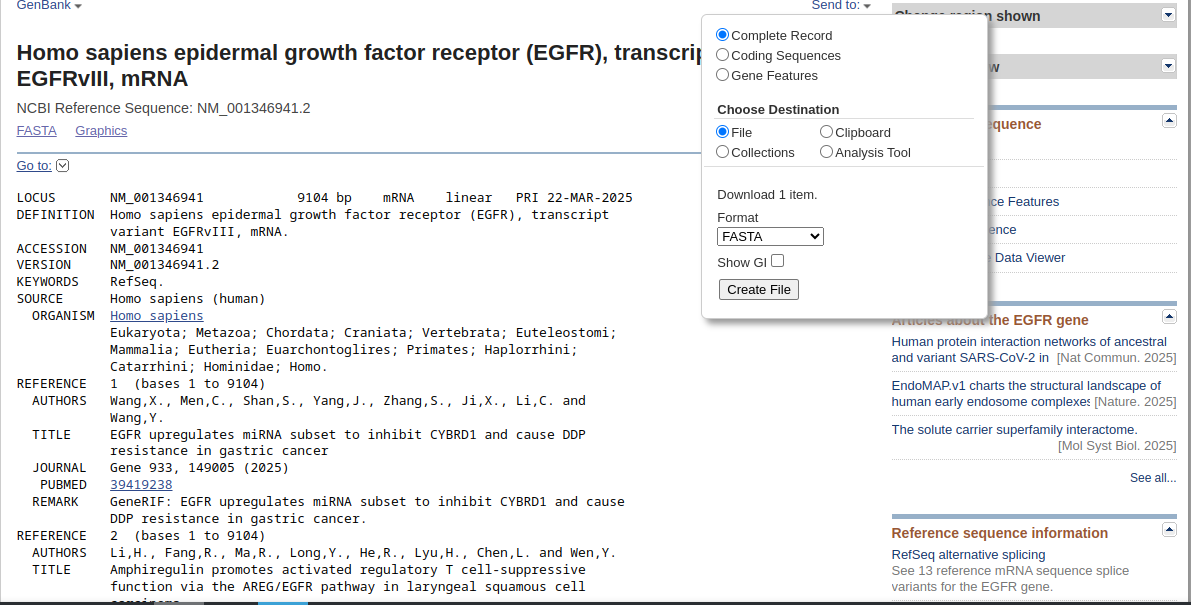
\includegraphics[scale=0.3]{Modul1/img/16.png}
            \end{enumerate}
    \end{flushleft}

    \begin{flushleft}
        \textbf{Materi 2 -  FASTA \& Handling File}
        \newline

        \begin{enumerate}
            \setlength\itemsep{2em}

            \item FASTA
            File FASTA adalah format yang sangat penting dalam dunia biologi molekuler
            dan bioinformatika. Format ini digunakan untuk menyimpan, berbagi, dan
            menganalisis informasi urutan nukleotida (DNA atau RNA) dan urutan asam
            amino (protein) yang merupakan komponen dasar kehidupan. File FASTA
            memiliki struktur sederhana yang memfasilitasi pemrosesan oleh komputer dan
            manusia.

            Struktur file FASTA berupa dua bagian yaitu, baris pertama itu berisi deskripsi dan baris berikutnya berisi urutan itu sendiri yang didahului oleh karakter $>$, dan baris kedua merupakan isi entri dari sequence record.
            \par\vspace{0.5cm}
            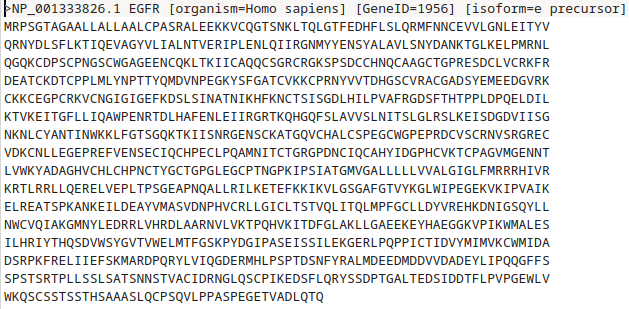
\includegraphics[scale=0.6]{Modul1/img/17.png}

            \item GenBank
            GenBank merupakan database sekuens nukleotida publik utama yang dikelola oleh National Center for Biotechnology Information (NCBI) yang menyimpan informasi sekuens DNA dan RNA dari berbagai organisme beserta anotasi biologisnya. Struktur file GenBank terdiri dari header yang berisi metadata seperti lokus (nama, panjang sekuens, jenis molekul), nomor aksesi, definisi, dan sumber organisme; bagian referensi yang mencantumkan publikasi ilmiah terkait; bagian features yang menguraikan anotasi biologis seperti gen, region pengkode protein (CDS), dan elemen regulasi dengan posisi spesifik; serta bagian origin yang menampilkan sekuens nukleotida aktual dalam format terstruktur. Pemakaian GenBank terutama dalam penelitian biologi molekuler untuk analisis sekuens gen, identifikasi homologi, prediksi fungsi gen, studi evolusi molekuler, dan sebagai referensi dalam proses annotasi genome berbagai spesies.

            \item Handling File FASTA
             Untuk menggunakan file FASTA pada Python perlu dilakukan handling file agar sekuens dapat dibaca oleh Python. Untuk pustaka yang digunakan untuk bioinformatika menggunakan biopython yang merupakan pustaka Python yang memiliki fungsi khusus untuk mengolah data biologi terutama sekuens seperti DNA dan Protein. Selain itu juga, aplikasi untuk pustaka ini bisa lebih luas lagi seperti pensejajaran sekuens, genetika populasi, struktur protein, filogenetika, motif sekuens, dan pembelajaran mesin.
             \begin{enumerate}
                 \item Handling file FASTA
                 \begin{lstlisting}[language=Python]
fasta = ''
with open('/content/AKTL.fasta','r') as handle:
    fasta = fasta.join([1.rstrip() for 1 in handle])
    handle.close()

print(fasta)
                 \end{lstlisting}
                \item Handling as SeqIO Object
                \begin{lstlisting}[language=Python]
from Bio import SeqIO

f = open('/content/AKT1.fasta', "r")
for i, fasta in enumerate(SeqIO.parse(f, 'fasta')):
   print((fasta.seq))

f.close()
                \end{lstlisting}
                \item Parsing SeqIO Object
                \begin{lstlisting}[language=Python]
from Bio import SeqIO

for _, seq_record in enumerate(SeqIO.parse("/content/AKT1.fasta", "fasta")):
   print(type(seq_record))
   print(seq_record)
                \end{lstlisting}
                \item Handling GenBank File
                \begin{lstlisting}[language=Python]
gb_file = '/content/EGFR.gb'
for gb_record in SeqIO.parse(open(gb_file,"r"), "genbank") :
   for record in gb_record.features:
       print(record)
                \end{lstlisting}
                \item Mencari bagian yang memiliki gen di dalamnya
                \begin{lstlisting}[language=Python]
gb_file = '/content/EGFR.gb'
for gb_record in SeqIO.parse(open(gb_file,"r"), "genbank") :
   for record in gb_record.features:
       if('gene' in record.qualifiers.keys()):
           print(record)
           print('==')
           print(record.qualifiers['gene'][0])
           print('==')
                \end{lstlisting}
             \end{enumerate}
        \end{enumerate}
    \end{flushleft}
\end{document}
